\documentclass{beamer}

\mode<presentation>
{
  \usetheme{Pittsburgh}
  \usecolortheme{seahorse}
  \usefonttheme{default}
  \setbeamertemplate{navigation symbols}{}
  \setbeamertemplate{caption}[numbered]
} 

\usepackage[english]{babel}
\usepackage[utf8]{inputenc}
\usepackage[T1]{fontenc}
\usepackage{kotex}

\usepackage{amsmath}
    \numberwithin{equation}{section}
\usepackage{amssymb}

\usepackage{hyperref}

\renewcommand{\theequation}{\arabic{equation}}

\usepackage{listings}
\usepackage{xcolor}

\definecolor{codegreen}{rgb}{0,0.6,0}
\definecolor{codegray}{rgb}{0.5,0.5,0.5}
\definecolor{codepurple}{rgb}{0.58,0,0.82}
\definecolor{backcolour}{rgb}{0.95,0.95,0.92}

\lstdefinestyle{mystyle}{
    backgroundcolor=\color{backcolour},   
    commentstyle=\color{codegreen},
    keywordstyle=\color{magenta},
    numberstyle=\tiny\color{codegray},
    stringstyle=\color{codepurple},
    basicstyle=\ttfamily\scriptsize,
    breakatwhitespace=false,         
    breaklines=true,                 
    captionpos=b,                    
    keepspaces=true,                 
    numbers=left,                    
    numbersep=5pt,                  
    showspaces=false,                
    showstringspaces=false,
    showtabs=false,                  
    tabsize=2
}

\lstset{style=mystyle}


\title{모델 훈련}
\author{박종민(jijupax@gmail.com)}
\date{May 19, 2020}

\begin{document}

\begin{frame}
    \titlepage
\end{frame}

% Uncomment these lines for an automatically generated outline.
% \begin{frame}{Outline}
%    \tableofcontents
% \end{frame}


\begin{frame}{학습 목표}

\begin{itemize}
\item 선형 회귀를 알아봅니다.
    \begin{itemize}
    \item 직접 계산할 수 있는 공식을 사용
    \item 경사 하강법을 사용
\end{itemize}
\vskip 0.25cm
\item 비선형 데이터셋을 훈련시킬 수 있는 다항 회귀를 알아봅니다.
\vskip 0.25cm
\item 과대접합을 감지하는 방법을 알아봅니다.
\vskip 0.25cm
\item 과대적합을 감소시킬 수 있는 규제 방법을 알아봅니다.
\vskip 0.25cm
\item 로지스틱 회귀와 소프트맥스 회귀를 알아봅니다.
\end{itemize}

\end{frame}

% ----------------------------------------

\begin{frame}{선형 회귀}

\begin{equation}
\begin{split}
\hat{y} &= \theta_{0} + \theta_{1}x_{1} + \theta_{2}x_{2} + \cdots + \theta_{n}x_{n} \\
        &= h_{\theta}(\mathbf{x}) = \mathbf{\theta} \cdot \mathbf{x}
\end{split}
\end{equation}

\vskip 1cm

\begin{itemize}
\item $\theta$는 선형 회귀 모델의 파라미터이고, 각 특성과 곱해집니다.
\vskip 0.25cm
\item 식 1과 같이 입력 특성의 가중치 합과 편향의 합으로 표현할 수 있습니다.
\end{itemize}

\end{frame}

% ----------------------------------------

\begin{frame}{회귀 모델 측정}

\begin{equation}
\textrm{MSE}(\mathbf{X}, h_{\theta}) = \dfrac{1}{m} \sum_{i=1}^{m} \left( \theta^{T}\mathbf{x}^{(i)} - y^{(i)} \right)^{2}
\end{equation}
    
\vskip 1cm

\begin{itemize}
\item 회귀 모델을 훈련시키는 방법은 식 2와 같이 비용 함수인 평균 제곱 오차(MSE)를 구해 그 값을 최소화하는 것입니다.
\end{itemize}

\end{frame}

% ----------------------------------------

\begin{frame}{정규방정식}

\begin{equation}
\hat{\theta} = \left( \mathbf{X}^{T} \mathbf{X} \right)^{-1} \mathbf{X}^{T} \mathbf{y}
\end{equation}

\vskip 1cm

\begin{itemize}
\item 비용 합수를 최소화하는 $\theta$를 찾기 위한 해적적인 방법을 식 3과 같이 정규방정식이라고 합니다.
\end{itemize}

\end{frame}

% ----------------------------------------

\begin{frame}{정규방정식}

\lstinputlisting[language=Python]{./scripts/normal_equation.py}

\vskip 1cm

\begin{itemize}
\item \texttt{numpy}를 사용하여 식 3을 직접 계산 하는 것이 가능합니다.
\vskip 0.25cm
\item \texttt{sklearn}의 \texttt{LinearRegression} 또는 \texttt{numpy.linalg.lstsq} 함수를 사용해도 됩니다.
\end{itemize}   

\end{frame}

% ----------------------------------------

\begin{frame}{경사 하강법}

\begin{block}{Gradient Descent}
비용 함수를 최소화하기 위해 반복해서 파라미터를 조정해가는 방법입니다.
\end{block}

\vskip 0.5cm

\begin{figure}
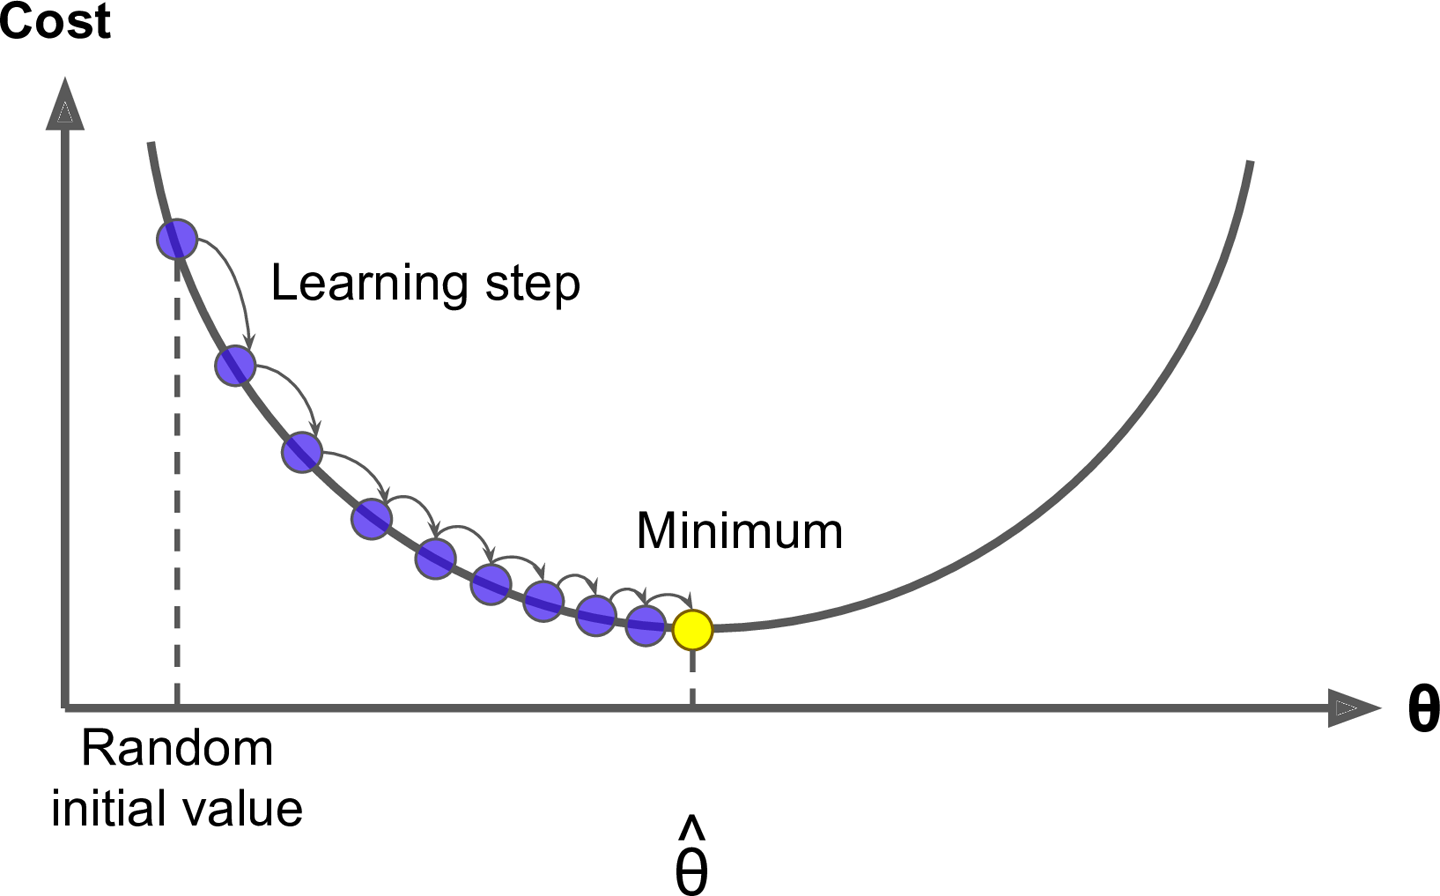
\includegraphics[width=20em]{./images/gradient_descent}
\caption{\label{fig:gradient_descent}경사 하강법}
\end{figure}

\end{frame}

% ----------------------------------------

\begin{frame}{경사 하강법}

\begin{itemize}
\item 파라미터 벡터 $\theta$에 대해 비용 함수의 현재 그레디언트를 계산하여 감소하는 방향으로 진행합니다.
\vskip 0.25cm
\item $\theta$를 임의의 값으로 시작해서 한 번에 조금씩 비용 함수가 감소되는 방향으로 진행합니다.
\vskip 0.25cm
\item 학습률의 크기에 따라 알고리즘의 수렴 속도가 틀리고, 클 경우 발산하거나 작을 경우 지역 최소값에 빠지기도 합니다.
\end{itemize}

\end{frame}

% ----------------------------------------

\begin{frame}{배치 경사 하강법}

\begin{equation}
\begin{split}
\dfrac{\partial}{\partial \theta_j} \text{MSE}(\boldsymbol{\theta}) &= \dfrac{2}{m}\sum\limits_{i=1}^{m}(\boldsymbol{\theta}^T \mathbf{x}^{(i)} - y^{(i)})\, x_j^{(i)} \\
\nabla_{\boldsymbol{\theta}}\, \text{MSE}(\boldsymbol{\theta}) &= \dfrac{2}{m} \mathbf{X}^T (\mathbf{X} \boldsymbol{\theta} - \mathbf{y})
\end{split}
\end{equation}

\begin{itemize}
\item 매 경사 하강법 스텝에서 전체 훈련 세트 $\mathbf{X}$에 대해 계산하는 방법입니다.
\vskip 0.25cm
\item 식 4는 배치 경사 하강법의 비용함수 그레디언트 벡터를 나타내는 것입니다.
\vskip 0.25cm
\item 경사 하강법의 스텝: $\boldsymbol{\theta}^{(\text{다음 스텝})}\,\,\, = \boldsymbol{\theta} - \eta \nabla_{\boldsymbol{\theta}}\, \text{MSE}(\boldsymbol{\theta})$
\end{itemize}

\end{frame}

% ----------------------------------------

\begin{frame}{확률적 경사 하강법}

\begin{itemize}
\item 매 스텝에서 딱 1개의 샘플을 무작위로 선택하여 그래디언트를 계산하는 방법입니다.
\vskip 0.25cm
\item 매우 적은 데이터를 처리하므로 배치 경사 하강법에 비해 훨씬 빠르고, 메모리를 적게 차지합니다.
\vskip 0.25cm
\item 무작위로 샘플을 선택하므로 전역 최소값 주변을 맴돌면서 수렵하게 됩니다.
\vskip 0.25cm
\item 학습 스케쥴을 조절하여 주변을 맴도는 문제를 해결할 수 있습니다.
\end{itemize}

\end{frame}

% ----------------------------------------

\begin{frame}{미니 배치 경사 하강법}

\begin{itemize}
\item 미니배치라고 부르는 임의의 작은 샘플 세트에 대해 그래디언트를 계산하는 방법입니다.
\vskip 0.25cm
\item 미니배치 크기를 적당히 조절하면 확률적 경사 하강법보다 덜 불규칙하게 수렴하게 됩니다.
\vskip 0.25cm
\item GPU를 사용한 병렬 계산에 유리한 방법입니다.
\end{itemize}
    
\end{frame}
    

% ----------------------------------------

\begin{frame}{경사 하강법 비교}

\begin{figure}
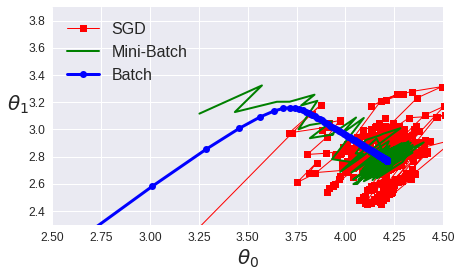
\includegraphics[width=25em]{./images/compare_gradient_descent}
\caption{\label{fig:compare_gradient_descent}파라미터 공간에 표시된 경사 하강법의 경로}
\end{figure}

\end{frame}

% ----------------------------------------

\begin{frame}{선형 회귀 알고리즘 비교}

\begin{table}
\centering
\tiny
\begin{tabular}{|l|l|l|l|l|l|}
\hline
알고리즘 & $m$이 클 때 & 외부 메모리 학습 지원 & $n$이 클 때 & 하이퍼파라미터 수 & 스케일조정 필요 \\ \hline \hline
정규방정식 & 빠름 & No & 느림 & 0 & No \\
SVD & 빠름 & No & 느림 & 0 & No \\
GD & 느림 & No & 빠름 & 2 & Yes \\
SGD & 빠름 & Yes & 빠름 & $\geq$2 & Yes \\
Mini-batch & 빠름 & Yes & 빠름 & $\geq$2 & Yes \\
\hline
\end{tabular}
\caption{\label{tab:compare_linear_regression_algorithm}선형 회귀를 사용한 알고리즘 비교}
\end{table}
    
\end{frame}

% ----------------------------------------

\begin{frame}{다항 회귀}

\begin{itemize}
\item 각 특성의 거듭 제곱을 새로운 특성으로 추가하여 확장된 특성을 포함한 데이터셋에 대해 선형 모델을 훈련 시키는 방법입니다.
\end{itemize}

\vskip 1cm

\lstinputlisting[language=Python]{./scripts/polynomial_regression.py}

\end{frame}

% ----------------------------------------

\begin{frame}{다항 회귀}

\begin{figure}
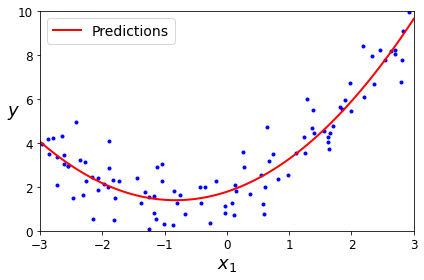
\includegraphics[width=20em]{./images/polynomial_regression}
\caption{\label{fig:polynomial_regression}다항 회귀 모델의 예측}
\end{figure}

\end{frame}

% ----------------------------------------

\begin{frame}{학습 곡선}

\begin{figure}
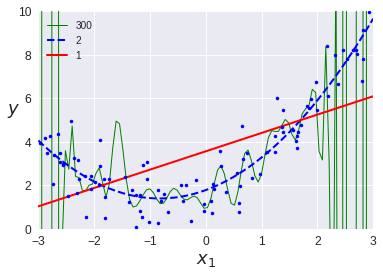
\includegraphics[width=20em]{./images/compare_polynomial_regression}
\caption{\label{fig:compare_polynomial_regression}고차 다항 회귀}
\end{figure}

\end{frame}

% ----------------------------------------

\begin{frame}{학습 곡선}

\begin{figure}
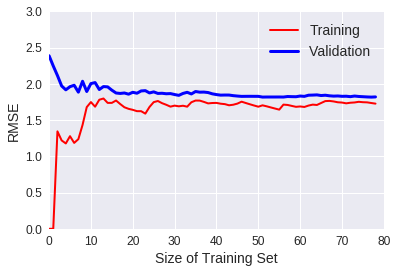
\includegraphics[width=20em]{./images/learning_curve_linear_regression}
\caption{\label{fig:learning_curve_linear_regression}선형 회귀 학습 곡선}
\end{figure}

\end{frame}

% ----------------------------------------

\begin{frame}{학습 곡선}

\begin{figure}
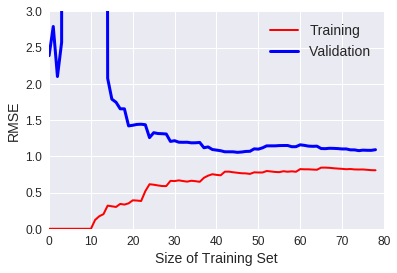
\includegraphics[width=20em]{./images/learning_curve_polynomial_regression}
\caption{\label{fig:learning_curve_polynomial_regression}다항 회귀 학습 곡선}
\end{figure}

\end{frame}

% ----------------------------------------

\begin{frame}{모델의 일반화 오차}

\begin{itemize}
\item 편향
\begin{itemize}
    \item 잘못된 가정으로 발생됩니다.
    \item 과소적합이 되기 쉬습니다.
\end{itemize}
\item 분산
\begin{itemize}
    \item 훈련 데이터에 있는 작은 변동에 모델이 과도하게 민감하기 때문에 발생합니다.
    \item 자유도가 높은 모델이 높은 분산을 가지기 쉬워 과대 적합 경향이 있습니다.
\end{itemize}
\item 줄일 수 없는 오차
\begin{itemize}
    \item 데이터 자체에 있는 노이즈 때문에 발생합니다.
    \item 데이터에서 노이즈를 제거하는 방법이 유일합니다.
\end{itemize}
\item 모델의 복잡도가 커지면 분산이 늘어나고 편향은 줄어듭니다.
\item 모델의 복잡도가 줄어들면 분산은 작아지고 편향이 커집니다.
\end{itemize}

\end{frame}

% ----------------------------------------

\begin{frame}{릿지 회귀}

\begin{equation}
J(\boldsymbol{\theta}) = \text{MSE}(\boldsymbol{\theta}) + \alpha \dfrac{1}{2}\sum\limits_{i=1}^{n}\theta_i^2
\end{equation}

\vskip 0.5cm

\begin{itemize}
\item 규제항 $\alpha \sum_{i=1}^{n}\theta_{i}^{2}$이 비용 함수에 추가된 것입니다.
\vskip 0.25cm
\item 규제항은 훈련하는 동안에만 비용 함수에 추가 되고, 테스트 시엔 사용하지 않습니다.
\vskip 0.25cm
\item $\alpha=0$이면 선형 회귀, $\alpha$가 아주 크면 모든 가중치가 거의 0에 가까워지고 데이터의 평균을 지나는 수평선이 됩니다.
\end{itemize}

\end{frame}

% ----------------------------------------

\begin{frame}{라쏘 회귀}

\begin{equation}
J(\boldsymbol{\theta}) = \text{MSE}(\boldsymbol{\theta}) + \alpha \sum\limits_{i=1}^{n}\left| \theta_i \right|
\end{equation}

\vskip 0.5cm

\begin{itemize}
\item Least Absolute Shrinkage and Selection Operator
\vskip 0.25cm
\item 규제항 $\alpha \sum_{i=1}^{n}\left|\theta_{i} \right|$이 비용 함수에 추가된 것입니다.
\vskip 0.25cm
\item 덜 중요한 특성의 가중치를 완전히 제거하는 특징이 있으므로 희소 모델을 만듭니다.
\end{itemize}

\end{frame}

% ----------------------------------------

\begin{frame}{라쏘와 릿지}

\begin{figure}
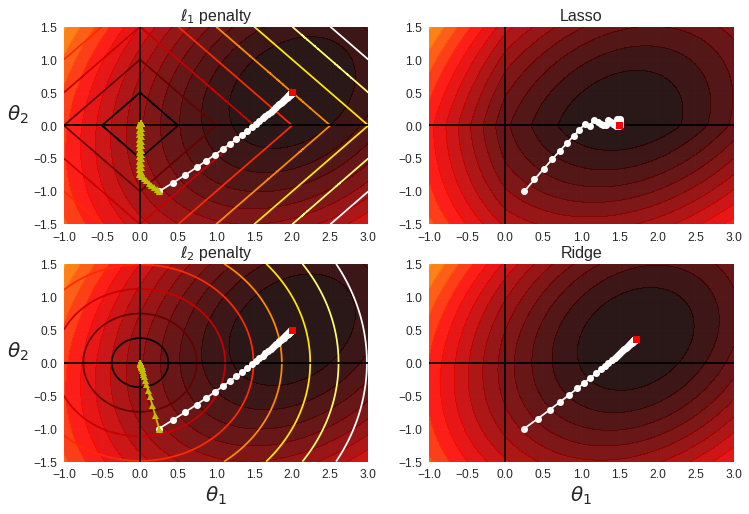
\includegraphics[width=25em]{./images/lasso_vs_ridge}
\caption{\label{fig:lasso_vs_ridge}라쏘 대 릿지 규제}
\end{figure}

\end{frame}

% ----------------------------------------

\begin{frame}{엘라스틱넷}

\begin{equation}
J(\boldsymbol{\theta}) = \text{MSE}(\boldsymbol{\theta}) + r \alpha \sum\limits_{i=1}^{n}\left| \theta_i \right| + \dfrac{1 - r}{2} \alpha \sum\limits_{i=1}^{n}{\theta_i^2}, \quad 0 \leq r \leq 1
\end{equation}

\vskip 0.5cm

\begin{itemize}
\item 릿지 회귀와 라쏘 회귀를 절충한 모델입니다.
\vskip 0.25cm
\item 혼합 비율 $r$을 사용해 조절하여 $r=0$이면 릿지 회귀이고 $r=1$이면 라쏘 회귀입니다.
\vskip 0.25cm
\item 릿지 회귀가 기본이 되지만 실제 쓰이는 특성이 몇 개뿐이라면 라쏘 회귀나 엘라스틱넷을 씁니다.
\vskip 0.25cm
\item 특성 수가 훈련 샘플 수보다 많거나 특성 몇개가 강하게 연관되어 있다면 엘라스틱넷을 씁니다.
\end{itemize}

\end{frame}

% ----------------------------------------

\begin{frame}{조기 종료}

\begin{itemize}
\item 검증 에러가 최소값에 도달하면 바로 훈련을 중지하는 방법입니다.
\vskip 0.25cm
\item 검증 에러가 증가하기 시작하면 과대 적합이 시작하는 것을 의미합니다.
\vskip 0.25cm
\item 검증 에러가 일정 시간 동안 최소값보다 크다는 확신이 들 때 학습을 멈추고 최소였을 때의 모델 파라미터로 되돌립니다.
\vskip 0.25cm
\item Beautiful free lunch, \emph{Geoffrey Hinton}
\end{itemize}

\end{frame}

% ----------------------------------------

\begin{frame}{조기 종료}

\begin{figure}
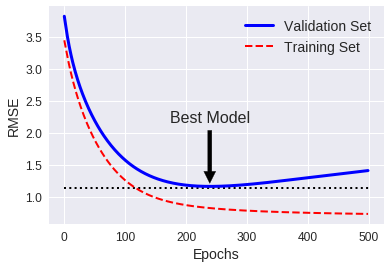
\includegraphics[width=20em]{./images/early_stopping}
\caption{\label{fig:early_stopping}라쏘 대 릿지 규제}
\end{figure}

\end{frame}

% ----------------------------------------

\begin{frame}{로지스틱 회귀}

\begin{itemize}
\item 샘플이 특정 클래스에 속할 확률을 추정하는데 사용합니다.
\vskip 0.25cm
\item 추정 확률이 50\%가 넘으면 모델은 그 샘플이 해당 클래스에 속한다고 예측합니다.(양성 클래스)
\vskip 0.25cm
\item 아니면 클래스에 속하지 않는다고 예측합니다.(음성 클래스)
\end{itemize}

\vskip 0.25cm

\begin{equation}
\hat{y} =
\begin{cases}
    0 & \hat{p} < 0.5 \text{일 때 } \\
    1 & \hat{p} \geq 0.5 \text{일 때 } 
\end{cases}
\end{equation}

\end{frame}
    
% ----------------------------------------

\begin{frame}{로지스틱 회귀}

\begin{equation}
\hat{p} = h_{\boldsymbol{\theta}}(\mathbf{x}) = \sigma(\boldsymbol{\theta}^T \mathbf{x})
\end{equation}

\begin{equation}
\sigma(t) = \dfrac{1}{1 + \exp(-t)}
\end{equation}

\begin{figure}
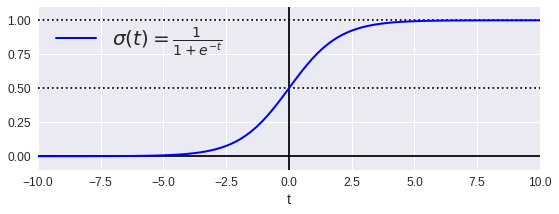
\includegraphics[width=20em]{./images/sigmoid}
\caption{\label{fig:sigmoid}시그모이드 함수}
\end{figure}

\end{frame}
% ----------------------------------------

\begin{frame}{로지스틱 회귀}

\begin{equation}
c(\boldsymbol{\theta}) =
\begin{cases}
    -\log(\hat{p}) & y = 1 \text{일 때 } \\
    -\log(1 - \hat{p}) & y = 0 \text{일 때 }
\end{cases}
\end{equation}

\begin{equation}
J(\boldsymbol{\theta}) = -\dfrac{1}{m} \sum\limits_{i=1}^{m}{\left[ y^{(i)} log\left(\hat{p}^{(i)}\right) + (1 - y^{(i)}) log\left(1 - \hat{p}^{(i)}\right)\right]}
\end{equation}

\begin{itemize}
\item 훈련의 목적은 $y=1$에 대해서 높은 확률을 추정하고, $y=0$에 대해서 낮은 확률을 추정하는 모델의 파라미터 벡터 $\theta$를 찾는 것입니다.
\item 정규방정식과 같은 로지스틱 회귀 비용 함수의 최소값을 계산하는 공식은 없습니다.
\item $J(\boldsymbol{\theta})$는 볼록 함수 이므로 경사 하강법으로 전역 최소값을 찾을 수 있습니다.
\end{itemize}

\end{frame}

% ----------------------------------------

\begin{frame}{소프트맥스 회귀}

\begin{equation}
s_k(\mathbf{x}) = ({\boldsymbol{\theta}^{(k)}})^T \mathbf{x}
\end{equation}

\begin{equation}
\hat{p}_k = \sigma\left(\mathbf{s}(\mathbf{x})\right)_k = \dfrac{\exp\left(s_k(\mathbf{x})\right)}{\sum\limits_{j=1}^{K}{\exp\left(s_j(\mathbf{x})\right)}}
\end{equation}

\begin{itemize}
\item 로지스틱 회귀 모델이 다중 클래스를 수행할 수 있도록 일반화된 것입니다.
\item 샘플 $\mathbf{x}$가 주어지면 각 클래스 $k$에 대한 점수 $S_K(\mathbf{x})$를 계산하고, 그 점수에 소프트맥스 함수를 적용하여 각 클래스의 확률을 추정합니다.
\item 한 번에 하나의 클래스만 예측 가능합니다.
\end{itemize}

\end{frame}

% ----------------------------------------

\begin{frame}{크로스 엔트로피}

\begin{equation}
J(\boldsymbol{\Theta}) = - \dfrac{1}{m}\sum\limits_{i=1}^{m}\sum\limits_{k=1}^{K}{y_k^{(i)}\log\left(\hat{p}_k^{(i)}\right)}
\end{equation}

\begin{equation}
\nabla_{\boldsymbol{\theta}^{(k)}} \, J(\boldsymbol{\Theta}) = \dfrac{1}{m} \sum\limits_{i=1}^{m}{ \left ( \hat{p}^{(i)}_k - y_k^{(i)} \right ) \mathbf{x}^{(i)}}
\end{equation}

\begin{itemize}
\item 모델이 타겟 클래스에 대해서 높은 확률을 추정하도록 만들기 위해 비용 함수를 최소화하는 전략으로 사용합니다.
\vskip 0.25cm
\item 크로스 엔트로피는 추정된 클래스의 확률이 타겟 클래스에 얼마나 잘 맞는지 측정하는 용도로 사용됩니다.
\end{itemize}

\end{frame}

% ----------------------------------------

\begin{frame}{결정 경계}

\begin{figure}
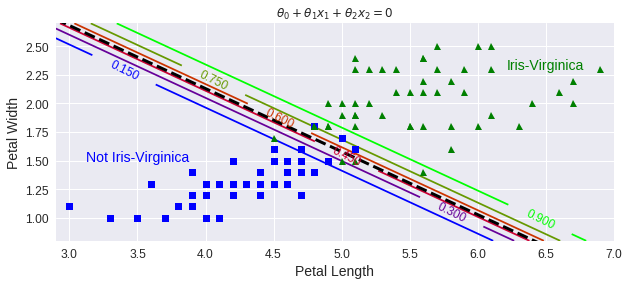
\includegraphics[width=25em]{./images/linear_decision_boundary}
\caption{\label{fig:linear_decision_boundary}선형 회귀 결정 경계}
\end{figure}

\end{frame}

% ----------------------------------------

\begin{frame}{결정 경계}

\begin{figure}
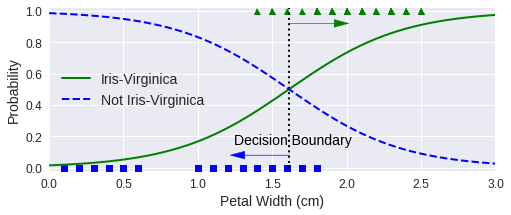
\includegraphics[width=25em]{./images/logistic_decision_boundary}
\caption{\label{fig:logistic_decision_boundary}로지스틱 회귀 결정 경계}
\end{figure}

\end{frame}

% ----------------------------------------

\begin{frame}{결정 경계}

\begin{figure}
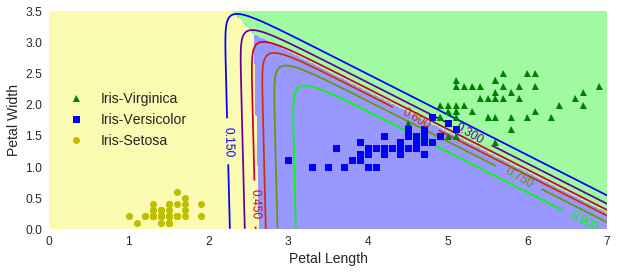
\includegraphics[width=25em]{./images/softmax_decision_boundary}
\caption{\label{fig:softmax_decision_boundary}소프트맥스 회귀 결정 경계}
\end{figure}

\end{frame}

% ----------------------------------------

\begin{frame}{참고 사항}

\begin{itemize}
\item 실습: https://github.com/rickiepark/handson-ml2
\vskip 0.5cm
\item 핸즈온 머신러닝 1판: https://bit.ly/2Tgfd2w
\end{itemize}

\end{frame}

% ----------------------------------------

\end{document}
